%% Example data sheet
%% Feel free to modify and use this file for any purpose, under
%% either the LaTeX Project Public License or under public domain.

% Options here are passed to the article class.
% Most common options: 10pt, 11pt, 12pt
\documentclass[10pt]{datasheet}

% Input encoding and typographical rules for English language
\usepackage[utf8]{inputenc}
\usepackage[english]{babel}
\usepackage[english]{isodate}
\usepackage[tocentry, tablegrid]{vhistory}

% tikz is used to draw images in this example, but you can
% also use \includegraphics{}.
\usepackage{tikz}
\usepackage{pgfplots}
\usepackage{circuitikz}
\usetikzlibrary{calc}

% These define global texts that are used in headers and titles.
\title{ETL Tamale Module Design}
\author{ETL Module design team}
\date{June 2022}
\revision{Revision 1}
\companylogo{\Huge CMS}

\begin{document}
\maketitle


\onecolumn

\begin{versionhistory}
	\vhEntry{1}{June, 2022}{C. Fangmeier}{Initial description based on Tamale module design presented at TIP in March 2022}
\end{versionhistory}

\begin{Large}
	\textbf{
    Disclaimer: This document comprises a snapshot in time of the evolution of the ETL module design. We anticipate no major changes from what is described here, but small adjustments here and there are expected.}
\end{Large}

\section{Overview of Design}

The ETL Module is built from a stack-up of a components as illustrated in Fig. \ref{fig:overview}. Starting from the bottom, the layers are:

\begin{itemize}
	\item A ceramic baseplate. Currently Alumina is the preferred material for its high thermal conductivity and relatively low cost compared to alternatives.
	\item An adhesive film. The leading candidate is an 80um thick silicone-based phase-change material. It serves as both a strong mechanical and low-resistance thermal interface between the silicon components and the baseplate.
	\item Four ETROC+LGAD subassemblies. These will be bump-bonded by an external vendor.
	\item A 2nd adhesive film. It will be the same material as the sensor-mount film, but cut to slightly different from the previous film.
	\item A PCB. This serves as the power and I/O interface between the readout board and the module via two board-to-board connectors. It also serves as a location to place any SMT passive components that must be placed very near the ETROCs.
\end{itemize}

The overall module dimensions are 56.5mm long by 43.1mm wide with an estimated stackup height of 2.97mm. For prototype modules to be constructed using ETROC2, the length is increased by 1mm to 57.5mm to ease the wirebonding process.


\begin{figure}[h]
	\centering
	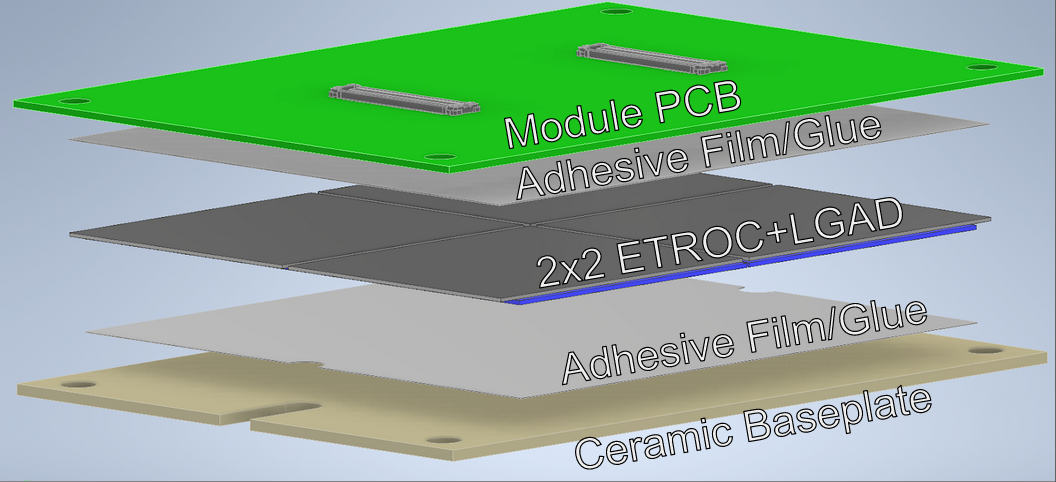
\includegraphics[width=\textwidth]{figures/overview.png}
	\caption{Stackup of ETL Module design}
	\label{fig:overview}
\end{figure}

This document is structured to follow the gantry-based assembly procedure while providing relevant details on the mechanical structure of the module and components along the way. A mechanical jig-based assembly is also being developed to be deployed as module factories that do not have gantries. The modules produced with either method will be identical.


\section{Module PCB}

Assembly begins with the Module PCB as the base layer of the stackup. It is important to note that the modules are built "upside down", i.e. PCB-side down, while they will be mounted baseplate-side down.

The Module PCB's dimensions match that of the module overall at 56.5x43.1mm. It has four 2.2mm diameter mounting holes, one in each corner. These are through holes for M2 screws that will serve to hold the assembly of the readout board and its several modules to the disc. The module PCB geometry is shown in Fig. \ref{fig:module-pcb} The PCB will be a 4-layer board with 0.5mm nominal thickness. The board-to-board connectors are JAE Electronics WP7B-S050VA1-R8000. These are surface-mount connectors with 50 connections each and an overall stacking height of 0.7mm. They are placed with a separation of 23.53mm centered on the top of the board. The top of the board will also potentially have a small number of surface-mount passive components as required by the ETROC.

\begin{figure}[h]
	\centering
	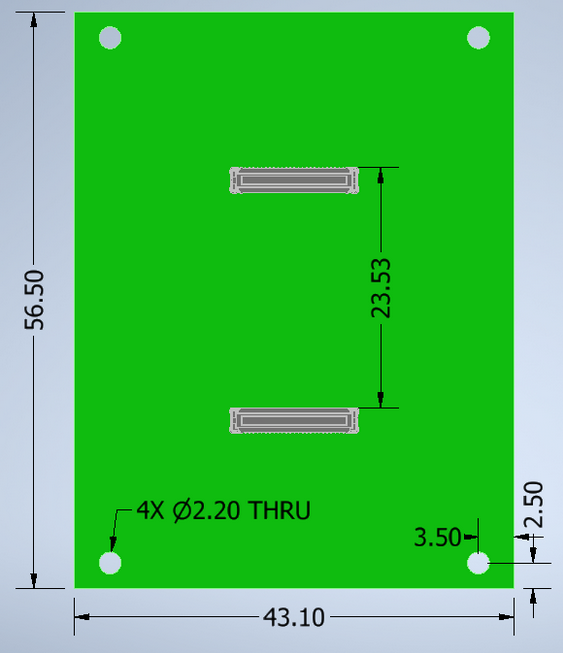
\includegraphics[width=0.5\textwidth,angle=-90]{figures/module_pcb.png}
	\caption{Geometry of Module PCB}
	\label{fig:module-pcb}	
\end{figure}

The opposite side of the board has a pattern of wire-bonding pads to connect with the ETROCs. This is described in more detail in a later section.



\section{Sensor-mount and Baseplate films}

As mentioned in the introduction, a set of adhesive films are used to mechanically attach the module layers together as well as provide a thermal path for removing heat from the ETROC and LGAD. The leading candidate material is Laird TPCM (Thermal Phase Change Material) 580(CHECK THIS). The film will be cut to shape by an outside vendor and will arrive to the module factories with plastic liners on each side with tabs to allow easy removal.

The sensor-mount film matches the envelope of the four ETROCs on the module. The dimensions are 42.6x46.6mm and 80um thick. The film will be applied to the Module PCB using a mechanical jig for alignment and to minimize the presence of trapped air between the film and the PCB.

A second film is applied to the baseplate and is used to fix the baseplate to the rest of the assembly. This film, the "Baseplate Film", is 43x43.4mm and has a 3mm diameter semicircular cutout centered along the shorter edge to provide access to the sensor for the bias wirebonds. This film will be applied to the baseplate using a similar jig to that used for applying the sensor-mount film. 

Immediately after placement, the subassemblies will be placed in a 60\degree C vacuum oven for a minimum of 20 minutes to cure the films. Curing the films causes them to conform to and better adhere to the surfaces they are in contact with. The first cure, or pre-assembly cure, is important to ensure that the films are well-adhered to the module PCBs and baseplates. Lacking this, there is a risk of the film shifting at any point up to the post-assembly cure.

\section{ETROC \& LGAD Subassembly}

The active components of the module, the ETL Read-out Chip, or ETROC, and the Low-gain Avalanche Diode (Detector?) sensor, will arrive at the module factories already bump-bonded together. The ETROC is 21x23mm and is 0.25mm thick. The LGAD consists of a 16x16 grid of pixels has overall dimensions of 21.4x21.6mm and is 0.3mm thick. The ETROC and LGAD are aligned such that the LGAD overhangs the edge of the ETROC on three sides by 0.2mm, and on the 4th side the ETROC extends past the sensor by 1.6mm with the wirebond pads along the edge. This is illustrated in Fig. \ref{fig:bbm-geometry}.

\begin{figure}[h]
	\centering
    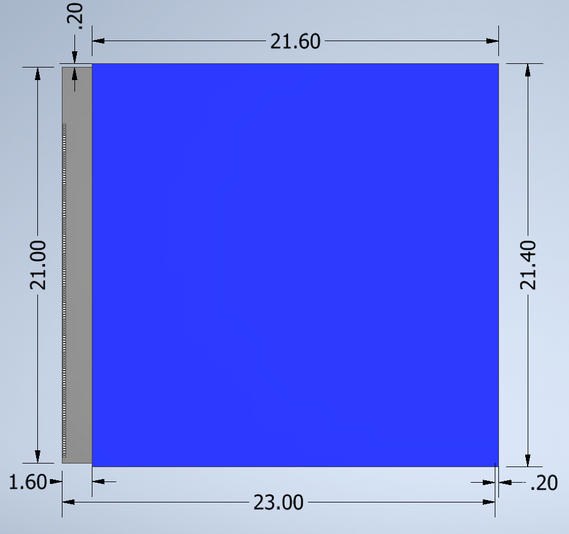
\includegraphics[width=0.5\textwidth]{figures/ETROCpLGAD.png}
    \caption{Geometry of ETROC+LGAD subassembly}
    \label{fig:bbm-geometry}	
\end{figure}

Each module has four ETROG+LGAD subassemblies. They are placed in a 2x2 array with a spacing of 0.2mm between adjacent sensors. The array is centered on the module PCB with each subassembly's wirebond pads facing out (Fig. \ref{fig:mod-with-bbms}).

\begin{figure}[h]
	\centering
	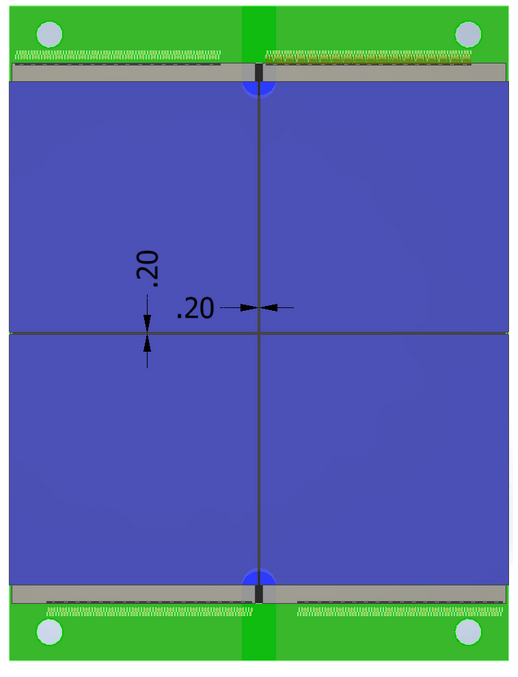
\includegraphics[width=0.5\textwidth,angle=90]{figures/module-with-bbms.png}
	\caption{Positioning of ETROC+LGAD subassemblies on the module PCB}
	\label{fig:mod-with-bbms}	
\end{figure}

The ETROC+LGAD subassemblies are placed onto a module PCB using a high-precision robotic gantry. Prior to pick-and-place the top plastic liner on the sensor-mount film on the module PCB is removed. The gantry is equipped with a vision system that measures the positions of the subassemblies with respect to the module PCB after placement. These measurements are used to check that the assembly precision meets requirements.

After placing the ETROC+LGAD subassemblies, the module is again placed in a vacuum oven for the post-assembly cure. This is needed to ensure that the subassemblies do not shift during wirebonding or encapsulation.


\section{Wirebonding}

Each ETROC requires 142 wirebonds to connect it to the module PCB. The pattern for these wirebonds is shown in \ref{fig:wirebonding-pattern}. In addition, bias voltage is supplied to the sensor via wirebonds that attach to its top surface. The ETROC and LGAD wirebonds both will be completed during the same stage of assembly. The bonding wire will be 25 um diameter aluminum-silicon alloy. The bond pads should have ENEPIG surface finish to achieve optimal wirebonding performance.


\begin{figure}[h]
	\centering
	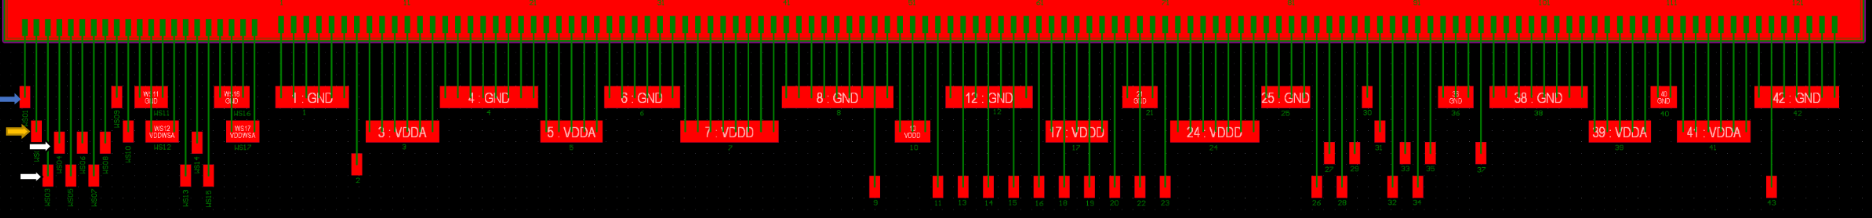
\includegraphics[width=\textwidth]{figures/wirebonding-pattern.png}
	\caption{Proposed wirebonding pattern for the ETROC}
	\label{fig:wirebonding-pattern}	
\end{figure}

\section{Wirebond Encapsulation}

It is important to encapsulate wirebonds with a suitable material to reduce the risk of physical damage, increase electrical isolation between the bonds, and damp any potential oscillations caused the Lorentz force on the wires in the magnetic field of CMS.

A suitable material that has been used extensively in CMS is Sylgard 186. It is a 2-part silicone elastomer that is dispensed over the wirebonds using a dedicated dispensing robot. At minimum, the encapsulant must cover the wirebond pads and feet, and full wire coverage is also being considered.

\section{Baseplate}

The final step in assembly is attaching the module baseplate. The baseplate is made of Alumina. It has overall dimensions matching the module PCB, but with a thickness of 1mm. The baseplate has a 2.5mm diameter hole in each corner. 

\begin{figure}[h]
	\centering
	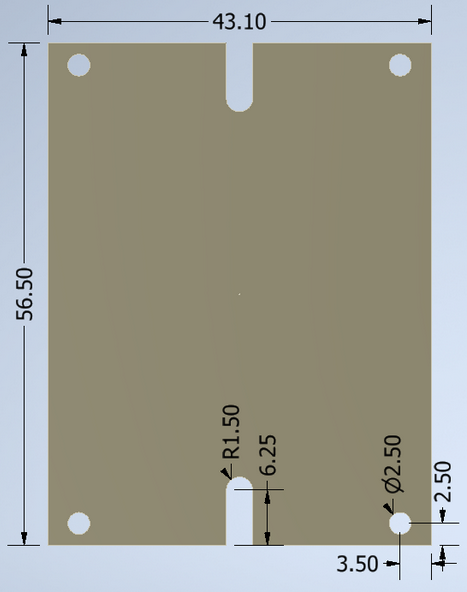
\includegraphics[width=0.5\textwidth,angle=-90]{figures/baseplate.png}
	\caption{Geometry of module baseplate}
	\label{fig:baseplate}	
\end{figure}

The baseplate also has a 3mm wide cutout centered along each of the the short ends that provides access for the bias wirebonds to the top surface of the sensor. This is shown in Fig. \ref{fig:baseplate-detail}.

\begin{figure}[h]
	\centering
	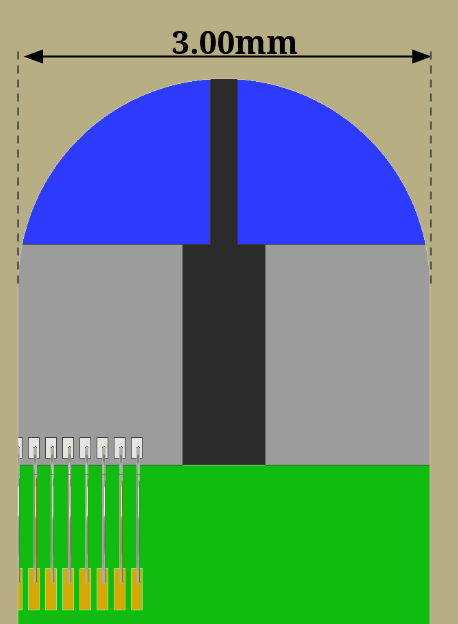
\includegraphics[width=0.2\textwidth]{figures/baseplate-detail.png}
	\caption{Detail of the baseplate cutout providing access to the sensor}
	\label{fig:baseplate-detail}	
\end{figure}

At this point in assembly a film has already been placed onto the baseplate and been pre-cured. What remains is to use the robotic gantry to place the baseplate on top of the module, and then perform the final film cure. At this point the module assembly is finished. After this, extensive testing and calibration will be performed on each module. A description of these tests is outside the scope of this document, but can be found in XXX.



\end{document}


